\section{Introduction}\label{section:intro}
The prediction of click-through rate (CTR) is critical in recommender system, where the task is to estimate the probability a user will click on a recommended item. In many recommender systems the goal is to maximize the number of clicks, and so the items returned to a user can be ranked by estimated CTR; while in other application scenarios such as online advertising it is also important to improve revenue, and so the ranking strategy can be adjusted as CTR$\times$bid across all candidates, where ``bid'' is the benefit the system receives if the item is clicked by a user. In either case, it is clear that the key is in estimating CTR correctly.

%and it is found quite beneficial to model the sophisticated feature interactions behind user behaviors (e.g., \cite{fm,pnn,wide-n-deep})
\begin{figure}[ht]
\setlength{\abovecaptionskip}{0pt}%
\setlength{\belowcaptionskip}{-10pt}
\centering
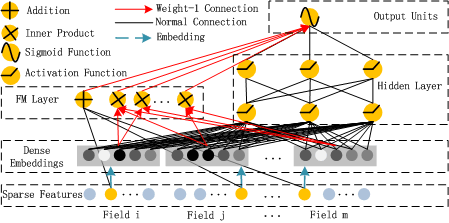
\includegraphics[width=0.45\textwidth]{img/architecture-deepfm.png}
\caption{\footnotesize{Wide \& deep architecture of DeepFM. The wide and deep component share the same input raw feature vector, which enables DeepFM to learn low- and high-order feature interactions simultaneously from the input raw features.}}\label{fig:architecture}
\end{figure}
It is important for CTR prediction to learn implicit feature interactions behind user click behaviors. By our study in a mainstream apps market, we found that people often download apps for food delivery at meal-time, suggesting that the (order-2) interaction between app category and time-stamp can be used as a signal for CTR. As a second observation, male teenagers like shooting games and RPG games, which means that the (order-3) interaction of app category, user gender and age is another signal for CTR. In general, such interactions of features behind user click behaviors can be highly sophisticated, where both low- and high-order feature interactions should play important roles. According to the insights of the Wide \& Deep model~\cite{wide-n-deep} from google, considering low- and high-order feature interactions \emph{simultaneously} brings additional improvement over the cases of considering either alone.

The key challenge is in effectively modeling feature interactions. Some feature interactions can be easily understood, thus can be designed by experts (like the instances above). However, most other feature interactions are hidden in data and difficult to identify \emph{a priori} (for instance, the classic association rule ``diaper and beer'' is mined from data, instead of discovering by experts), which can only be captured \emph{automatically} by machine learning. Even for easy-to-understand interactions, it seems unlikely for experts to model them exhaustively, especially when the number of features is large.

%Below we review previous efforts in learning feature interaction and then summarize our contributions.
%%\subsection{Background}\label{section:intro:back}
%Existing methods can be divided into three categories: ``wide'' models, which capture low-order feature interactions; deep models, which capture high-order feature interactions; and the latest Wide \& Deep models, which capture both low- and high-order feature interactions.
%

%\subsubsection{Wide models}
Despite their simplicity, generalized linear models, such as \emph{FTRL}~\cite{FTRL}, have shown decent performance in practice. However, a linear model lacks the ability to learn feature interactions, and a common practice is to manually include pairwise feature interactions in its feature vector. Such a method is hard to generalize to model high-order feature interactions or those never or rarely appear in the training data~\cite{fm}. \emph{Factorization Machines (FM)}~\cite{fm} model pairwise feature interactions as inner product of latent vectors between features and show very promising results. While in principle FM can model high-order feature interaction, in practice usually only order-2 feature interactions are considered due to high complexity.

%GBDT~\cite{GBDT}, random forest~\cite{RF} are two different Tree ensemble models. They are also proposed to explore unseen feature interactions, however, these models are still unable to fully explore useful feature patterns due to the limit of the model expressiveness.


%\subsubsection{Deep models}
As a powerful approach to learning feature representation, deep neural networks  have the potential to learn sophisticated feature interactions. Some ideas extend CNN and RNN for CTR predition \cite{cnn,rnn}, but CNN-based models are biased to the interactions between neighboring features while RNN-based models are more suitable for click data with sequential dependency. \cite{fnn} studies feature representations and proposes \emph{Factorization-machine supported Neural Network (FNN)}. This model pre-trains FM before applying DNN, thus limited by the capability of FM. Feature interaction is studied in \cite{pnn}, by introducing a product layer between embedding layer and fully-connected layer, and proposing the \emph{Product-based Neural Network} (\emph{PNN}). As noted in~\cite{wide-n-deep}, PNN and FNN, like other deep models, capture little low-order feature interactions, which are also essential for CTR prediction. To model both low- and high-order feature interactions, \cite{wide-n-deep} proposes an interesting hybrid network structure (\emph{Wide \& Deep}) that combines a linear (``wide'') model and a deep model. In this model, two different inputs are required for the ``wide part'' and ``deep part'', respectively, and the input of ``wide part" still relies on expertise feature engineering.



One can see that existing models are biased to low- or high-order feature interaction, or rely on feature engineering. In this paper, we show it is possible to derive a learning model that is able to learn feature interactions of all orders in an end-to-end manner, without any feature engineering besides raw features. Our main contributions are summarized as follows:
\begin{itemize}
\item We propose a new neural network model DeepFM (Figure~\ref{fig:architecture}) that integrates the architectures of FM and deep neural networks (DNN). It models low-order feature interactions like FM and models high-order feature interactions like DNN. Unlike the wide \& deep model~\cite{wide-n-deep}, DeepFM can be trained end-to-end without any feature engineering.
\item DeepFM can be trained efficiently because its wide part and deep part, unlike~\cite{wide-n-deep}, share the same input and also the embedding vector. In ~\cite{wide-n-deep}, the input vector can be of huge size as it includes manually designed pairwise feature interactions in the input vector of its wide part, which also greatly increases its complexity.
\item We evaluate DeepFM on both benchmark data and commercial data, which shows consistent improvement over existing models for CTR prediction.
\end{itemize}


